\documentclass[prez_parietal.tex]{subfiles}
\begin{document}



\begin{frame}[t]
\frametitle{Vectorized model}
    \begin{columns}
        \column{.5\textwidth}
        \begin{itemize}\itemsep1em
            \item $x$ is a vector in $\Rset^T$
            \item $\epsilon$ is a noise vector in $\Rset^T$  
            \item $D$ is a matrix in $\Rset^{T\times LK}$
            \item $z$ is a coding vector in $\Rset^{LK}$ 
        \end{itemize}
        \column{.5\textwidth}
        {\bf Sparse Linear model:}
        \begin{align*}
        x & = Dz + \epsilon \phantom{ \sum_{k=1}^K }
        \end{align*}
        \vskip.5em
        with \makebox[1em]{$z$} sparse.\\{\color{gray} Few of its coefficients are non-zero.}
    \end{columns}
    \vskip1em
    \scriptsize\centering
    \inputTikZ{.4}{vectorial_dictionary}.\\
\end{frame}

%------------------------------------------------------------------------
\subsection{Motivations}
%------------------------------------------------------------------------



\begin{frame}[t]{Adaptive Optimization}

	We have to solve $N$ problems with a common structure $\pmb D$.\\
	\[
		Z^{[n],*} = \argmin_{Z^{[n]}}\| X^{[n]} - \sum_{k=1}^K\pmb D_k *  Z_k^{[n]}\|_2^2
				+ \lambda\| Z^{[n]}\|_1
	\]
	{\textbf{Can we use this structure to accelerate the resolution?}\\[1em]}
	\visible<2->{
		Yes, with the Learned ISTA \cite{Gregor10}
	}

{
	\only<2>{
		\begin{figure}
		\begin{subfigure}[b]{.47\textwidth}
			\centering
			\inputTikZ{.7}{ista_tikz.tex}
			\mbox{\hskip-2em\inputTikZ{.5}{lista_tikz.tex}}
		\end{subfigure}
		\begin{subfigure}[b]{.47\textwidth}
			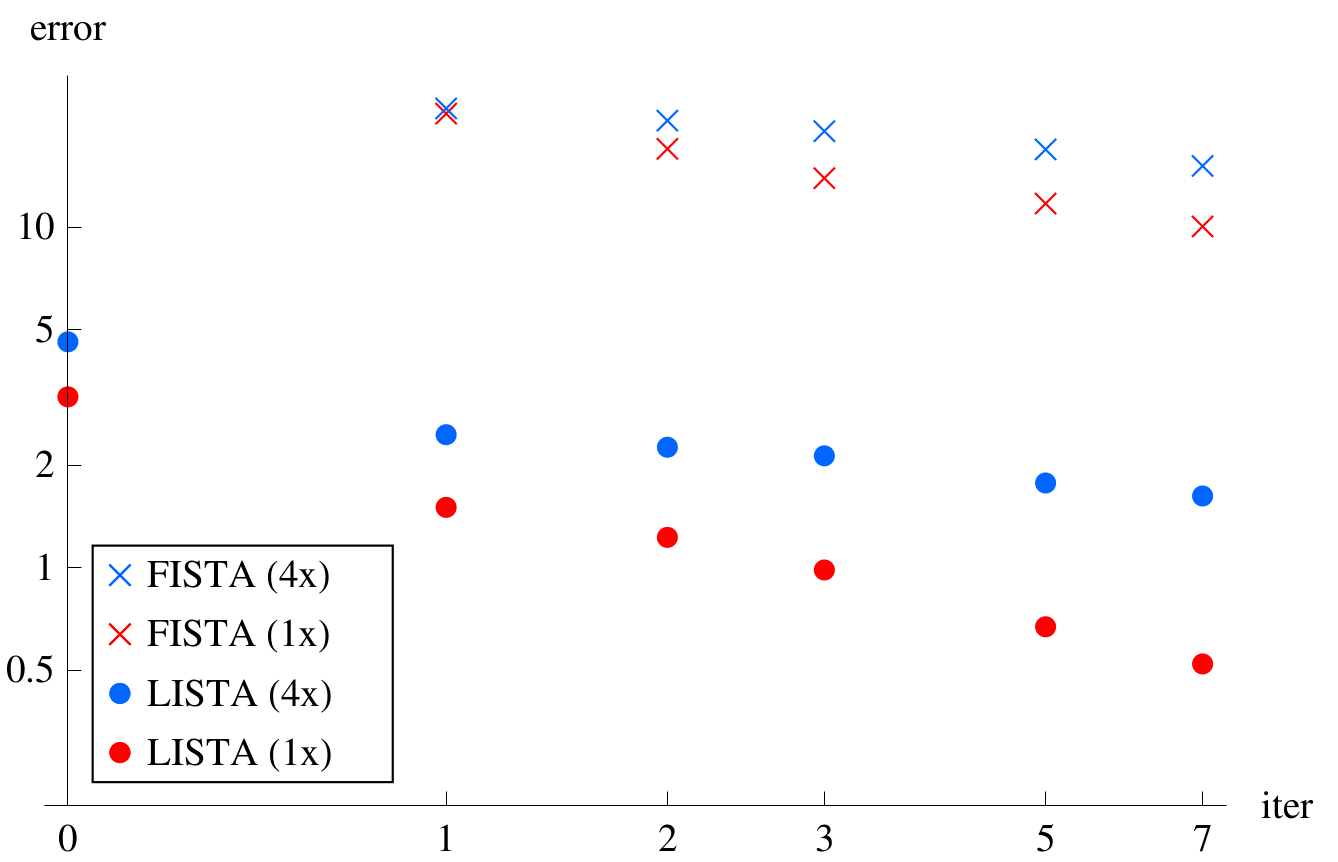
\includegraphics[width=.8\textwidth]{Gregor10}
		\end{subfigure}\\
		%\caption*{Adapted from \cite{Gregor10}}
		\end{figure}
	}
	\only<3>{
	\vskip1.5em
		\textbf{Open problem: Why does it work?}\\
		\begin{itemize}
			\item Can we leverage the structure of $\pmb D$?
			\item Can we get a non-asymptotic acceleration of ISTA?
			\item How to explain LISTA performance?
		\end{itemize}
		\mycite{Giryes2016, xin2016maximal}
	}
}
\end{frame}

\begin{frame}{Notations}
	Consider the sparse coding problem with a dictionary $D$.\\[.5em]
	\[
		z^{*} = \argmin_{z} F(z) = 
				\underbrace{\| x - D z\|_2^2}_{E(z)}
				+ \lambda\| z\|_1
	\]
	We denote $B = D\tran D$ is the Gram matrix of $D$.\\[1em]
	
	\textbf{We introduce a novel class of algorithms -- FacNet -- based on a sparse factorization of $B$.}
	
	\vskip1em
		Quadratic form: $Q_S(u, v) = \frac{1}{2}(u-v)\tran S (u-v) + \lambda \|u\|_1~.$\\[1em]
		
		Note that $F(z) = Q_B(z, D^\dagger x)$\\[1em]
		For $S$ is diagonal, $\argmin_u Q_S(u, v)$ can be efficiently minimized as
		the problem is separable on each coordinate.
\end{frame}



%----------------------------------------------------------------
\subsection{Adaptive ISTA: FacNet}
%----------------------------------------------------------------


\begin{frame}[t]{Toward an adaptive procedure \mycite{Moreau2017}}
	\vskip1em
	Given an estimate $z^{(q)}$ of $z^*$ at iteration $q$, we can write:
	\begin{eqnarray*}
		F(z) & =& E(z) + \lambda\|z\|_1\\
		     & = & E(z^{(q)}) + \left\langle \nabla E(z^{(q)}) , z-z^{(q)} \right\rangle
						+ Q_{\makebox[.7em][c]{$B$}}(\phantom{\bf A}z, \phantom{\bf A}z^{(q)})~,\\
	\end{eqnarray*}%
	\vskip-1em
	\only<1>{\color{lightblue!70}}%
	\uncover<2->{\underline{ISTA:} ~~~~~Replace $B$ by diagonal matrix $S = \|B\|_2\pmb I_K$ \\[.5em]}
	\uncover<3->{\underline{\bf FacNet:} ~~Replace $B$ by $A\tran S A$ ~~~($S$ diagonal, $A$ unitary)}
	\only<-2>{\color{black}}\\
	\vskip-.5em
	\def\surogate{\alt<2>{F_q(z)}{\widetilde F_q(z)}}
	\begin{eqnarray*}
	\only<2->{
		\surogate{} & = & E(z^{(q)}) + \left\langle \nabla E(z^{(q)}) , z-z^{(q)} \right\rangle
						+ Q_{\color{blue!75}\pmb S\visible<3->{_q}}
							(\visible<3->{{\color{blue!75}\pmb A_q}}z, \visible<3->{{\color{blue!75}\pmb A_q}}z^{(q)})~,\\
			   \min_z \surogate{} &\Leftrightarrow& \min_z Q_{S\visible<3->{_q}}\Big(\visible<3->{A_q}z, \visible<3->{A_q}z^{(q)}
			   	- \text{\makebox[2.5em][c]{$S^{-1}\alt<2>{}{_qA_q}$}}\nabla E(z^{(q)})\Big)
	}
	\end{eqnarray*}
	\uncover<4>{
	Can we choose $A_q, S_q$ to accelerate the optimization compared to ISTA?}

	
\end{frame}
\begin{frame}{Toward and adaptive procedure}
		\centering
		\hskip2em
		\makebox[.75\textwidth][c]{
		\only<1>{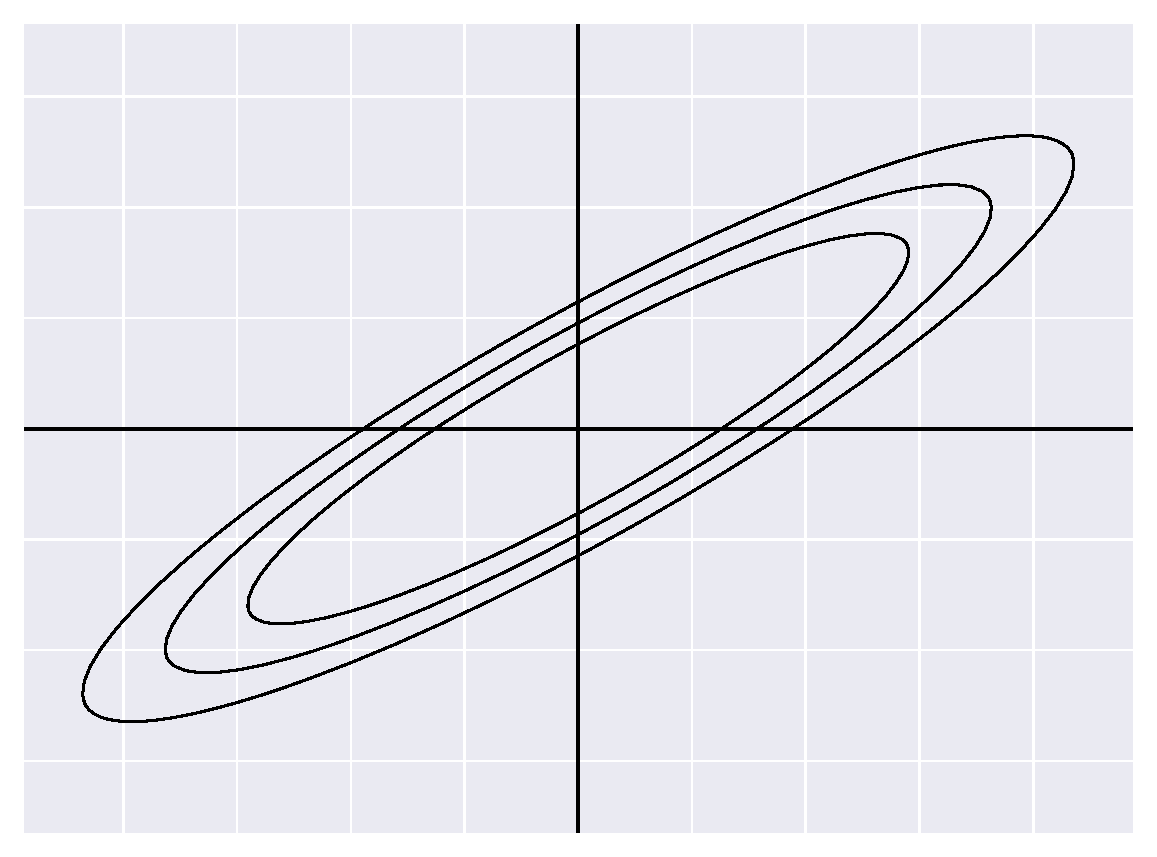
\includegraphics[height=.75\textheight]{ell1}}%
		\only<2>{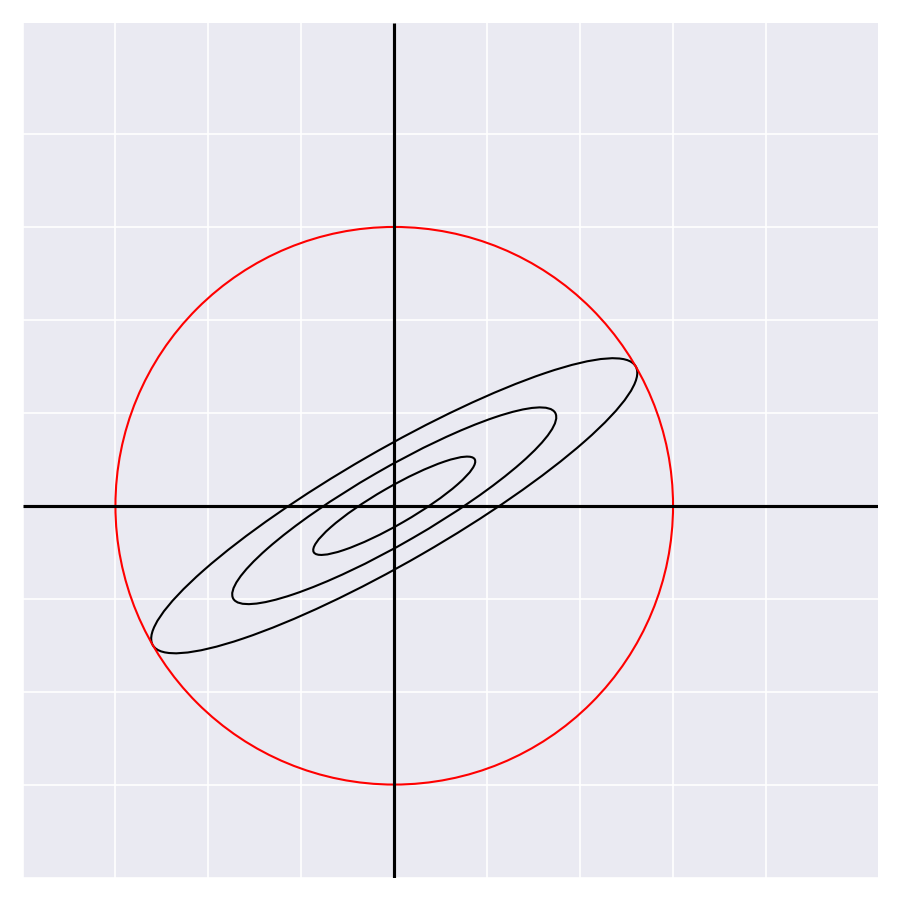
\includegraphics[height=.75\textheight]{ell2}}%
		\only<3->{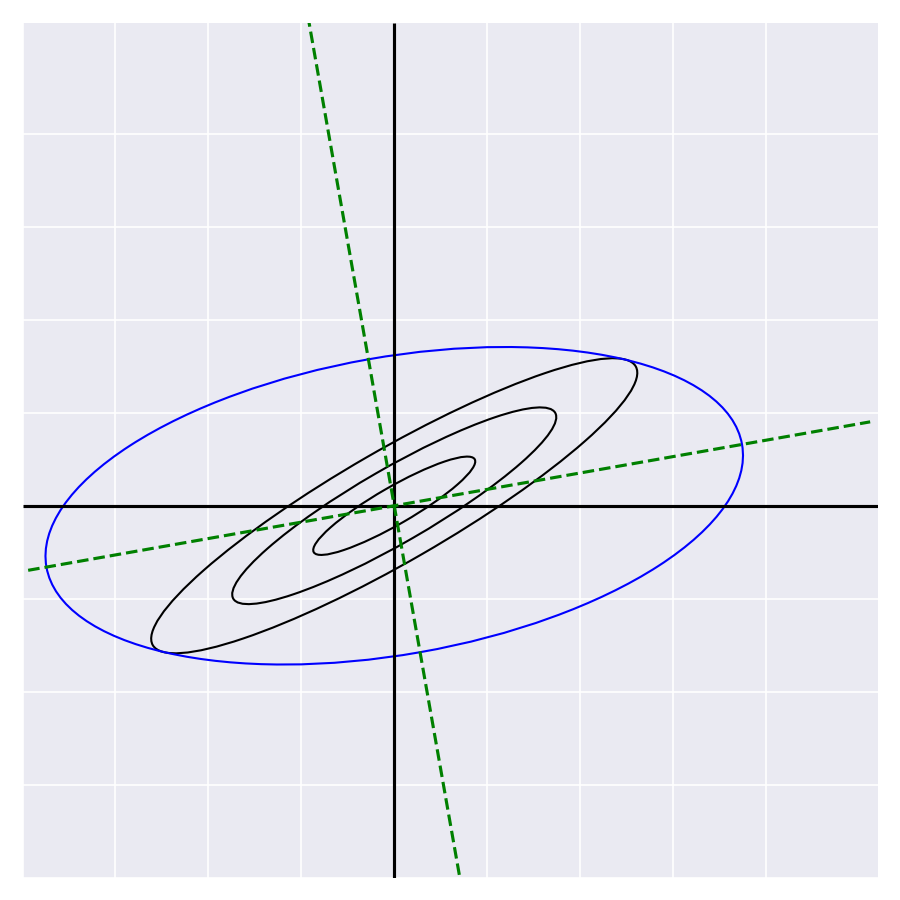
\includegraphics[height=.75\textheight]{ell3}}
		}\\

\end{frame}


\begin{frame}{Toward an adaptive procedure}

	Similar iterative procedure with steps adapted to the problem topology.
	\[
		\widetilde{F_q}(z) = F(z) + (z-z^{(q)})\tran R(z-z^{(q)}) + \delta_A(z)
	\]
%\textbf{Proximal resolution :}
%\[z^{(q+1)} = \argmin_z F(z) = E(z^{(q)}) + \langle B(z^{(q)}-y) , z-z^{(q)} \rangle + \frac{1}{2}\| z - z^{(q)} \|_B^2 + G(z)~ ,\]
%$\color{darkblue}\Rightarrow$ Not computationally efficient but quick minimization.\\[1.5em]


	Tradeoff between:\\[.3em]
	\begin{itemize}\itemsep1em
		\item Rotation to align the norm $\|\cdot\|_B$ and the norm $\|\cdot\|_1$~,
		\keypoint{Computation}
		\[ R = A\tran SA - B\]
		\item Deformation of the $\ell_1$-norm with the rotation $A$~.
		\keypoint{Accuracy}
		\[ \delta_A(z) = \lambda\left(\|Az\|_1-\|z\|_1\right) \]
	\end{itemize}
\end{frame}
\begin{frame}{One step improvement}
		Suppose that $R = A\tran S A - B \succ 0$ is positive definite, and define 
		\[z^{(q+1)} = \arg\min_z \widetilde{F_q}(z)~,\]
		Then
		\[
		\begin{split}
			F(z^{(q+1)}) - F(z^*) \leq \frac{1}{2}(z^{(q)} - z^*)\tran R (z^{(q)} - z^*)~~~~~\\
									+ \delta_A(z^*) - \delta_A(z^{(q+1)})~.
\end{split}
		\]
	\vskip1em
	We are interested in factorization $(A, S)$ for which $\|R\|_2$ and $\delta_A$  are small.
\end{frame}



\begin{frame}{Theoretical results}
    \begin{itemize}\itemsep1em
		\item We showed that FacNet has the same asymptotic convergence rate as ISTA
		in $\mathcal O(\tfrac{1}{q})$.
		\item The constant factors are different and can be improved.
		If the factorization $(A_q, S_q)$ at iteration $q$  verifies
			\[
				\|R_q\|_2 + 2 \frac{L_{A_q}(z^{(q+1)})}{\|z^*-z^{(q)}\|_2} \le \frac{\|B\|_2}{2}
			\]
			and $A_p = \pmb I_K, S_p = \|B\|_2\pmb I_K$ for $p > q$, then the procedure has
			improved convergence rate compared to ISTA.\\[1em]
			{{\usebeamercolor[fg]{block title}$\Rightarrow$}} There is a phase transition when
			 $\|z^{(q)} - z^*\|_2 \to 0$
	\end{itemize}
\end{frame}



%---------------------------------------------------------
\subsection{Understanding LISTA}
%---------------------------------------------------------

\begin{frame}{Learned ISTA \mycite{Gregor10}}
	\vskip1em
		\centering
		\inputTikZ{.8}{ista_tikz.tex}\\
		\inputTikZ{.8}{lista_tikz.tex}\\
		Network architecture for ISTA/LISTA. LISTA is the unfolded version
				 of the RNN of ISTA, trainable with back-propagation.
	\vskip1em
	With $W_e = \frac{D\tran}{\|B\|_2} $ and $W_g = I - \frac{B}{\|B\|_2}$, this network computes exactly 2 iterations of ISTA.
	
\end{frame}
\begin{frame}{FacNet}
	Specialization of LISTA
		\[
			z^{(q+1)} = A\tran \prox_{S}( Az^{(q)} - S^{-1}A B(z^{(q)} - y))~,
		\]
		with $A$ unitary and $S$ diagonal.\\
	Same architecture with more constraints on the parameter space:
	\begin{equation*}
	\begin{cases}
		W_e & = S^{-1}A D\tran\\
		W_g & =  A\tran - S^{-1}A BA\tran
	\end{cases}
	\end{equation*}
	\vskip2em
	\hskip3em $\Rightarrow$ LISTA can be at least as good as this model.
\end{frame}



\begin{frame}{Generic Dictionary}
	\vskip1em
	\begin{itemize}\itemsep1em
		\item Generic dictionary uniformly sample in unit ball,
		\[
			D \sim \mathcal S^{p-1}~,
		\]
		\item Sparse code generated with Bernouilli-Gaussian model, \emph{s.t.}
		\[z_k = b_ka_k, \hskip2em b_k \sim \mathcal B(\rho) \text{ and } a \sim \mathcal N(0, \sigma \pmb I_K)\]
	\end{itemize}
	\vskip1em 
	\emph{Fixed: } $K = 100$, $P = 64$, $\sigma = 10$ and $\lambda = 0.01$
\end{frame}

\begin{frame}{Generic Dictionary}
		\centering
		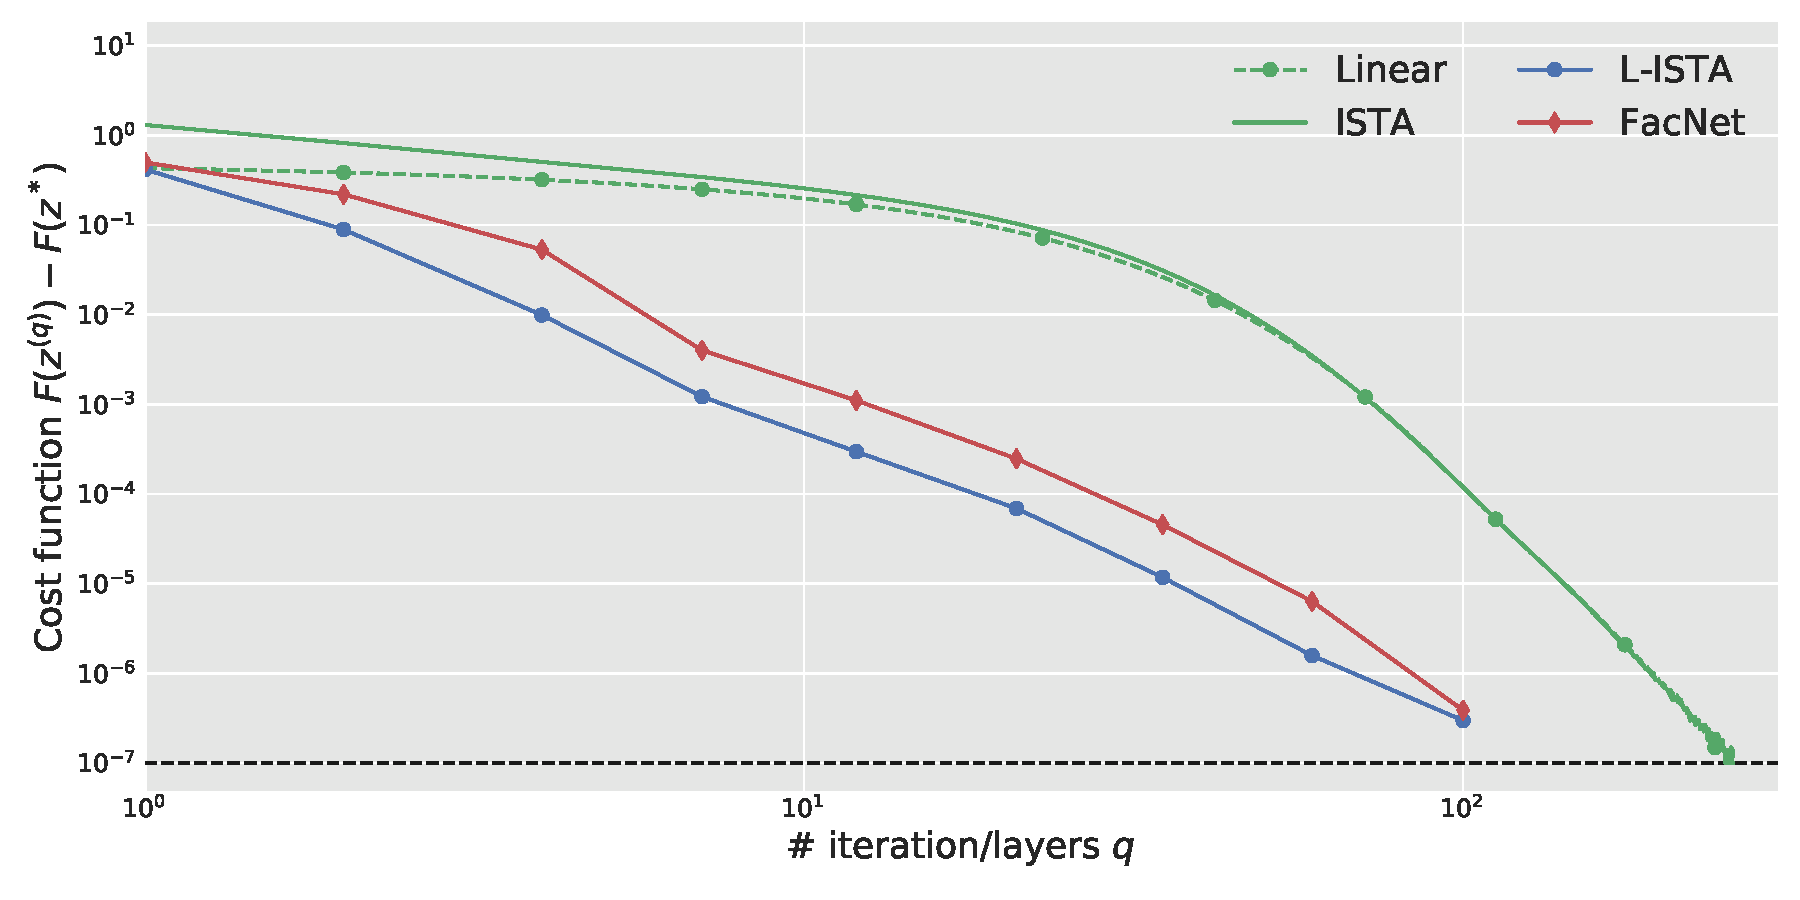
\includegraphics[width=\textwidth]{curve_sparse005_seaborn_min}\\
		$\rho = {}^1/_{20}$.\\[1em]

%	\only<2>{
%		\includegraphics[width=\textwidth]{curve_sparse02_seaborn_min}\\
%		$\rho = {}^1/_{4}$.\\[1em]
%	}
		Evolution of the cost function $F(z^{(q)}) - F(z^*)$ with the number
	   	of layers/iterations $q$ with a denser model
\end{frame}




\begin{frame}{Adversarial dictionary}
		\vskip2em
		The dictionary is constructed such that it eigen-vectors are sampled from the
		Fourier basis, with
		\[
			D_{k, j} = e^{-2i\pi k \zeta_j}
		\]
		for a random subset of frequencies
		\[
			\left \{ \zeta_i \right \}_{0\le i \le p} \sim \mathcal U \left\{\frac{m}{K}; 0 \le m \le \frac{K}{2}\right\}
		\]
		Diagonalizing $B$ implies large deformation of the $\ell_1$-norm. 

\end{frame}

\begin{frame}{Adversarial dictionary}
	%\vskip4em
\centering
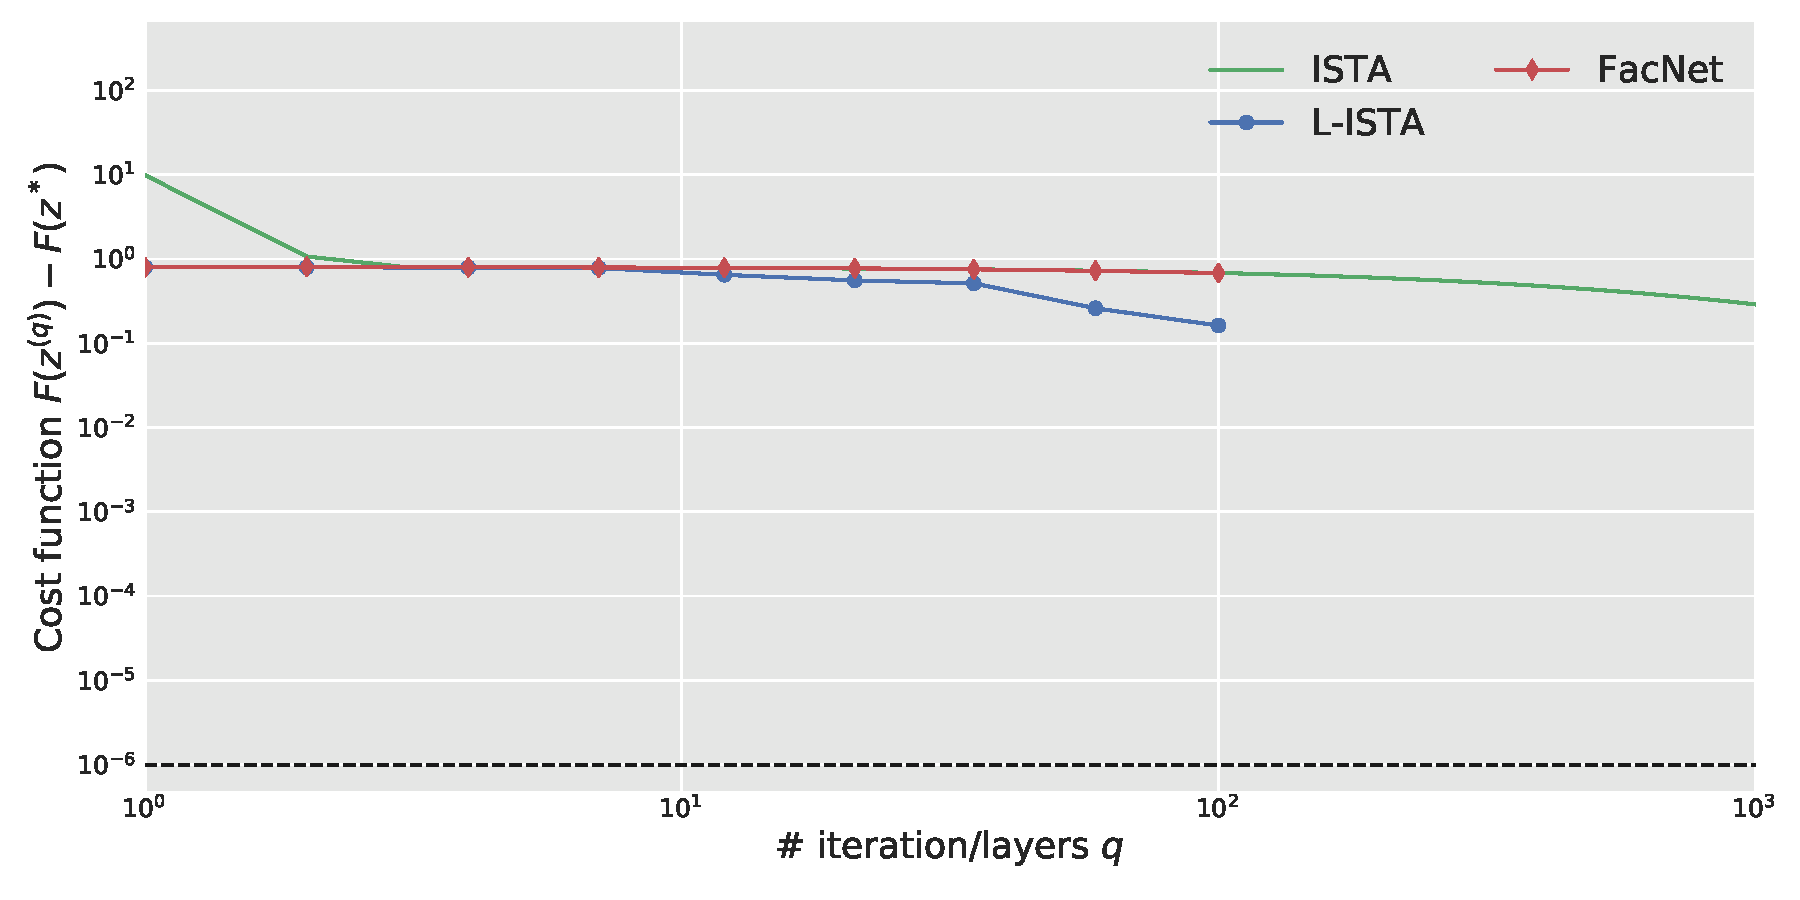
\includegraphics[width=\textwidth]{curve_adverse_seaborn_min}\\
    Evolution of the cost function $F(z^{(q)}) - F(z^*)$ with the number of layers/iterations $q$ 
    with an adversarial dictionary.
\end{frame}


\begin{frame}{Contribution}

	\textbf{Contributions}
	\begin{itemize}
		\item \underline{Theoretical analysis:} Non asymptotic acceleration of ISTA is possible
		based on the structure of $\pmb D$,
		\item \underline{FacNet Algorithm:} Sufficient analysis to explain LISTA acceleration,
		\item \underline{Adversarial Example:} Empirically showed the structure of $D$ is necessary
		for LISTA. 
	\end{itemize}

	\vskip1em
    \textbf{Future work}
	\begin{itemize}
	    \item Direct factorization: Improve the factorization formulation
	    for direct optimization,
	    \item Adaptation of the analysis to convolutional sparse coding,
	    \item Sparse PCA: Link the sparse eigenvectors properties to our factorization.
    \end{itemize}
	
\end{frame}





\biblio{}
\end{document}